
\chapter{Week5}

\section{Wednesdays}\index{week5_Tuesday_lecture}
Today we will discuss topics about differentiation. Note that the topics in Friday will be more difficult.
\subsection{Differentiation}
\paragraph{Notations and Conventions}
Given two functions $\phi$ and $\xi$, then we denote $\phi(x)=O(\xi(x))$ near $x_0$ if there exists a constant $C$ such that
\[
\left|\frac{\phi(x)}{\xi(x)}\right|\le C\mbox{ for $x$ near $x_0$},
\]
i.e., $|\phi(x)|\le C|\xi(x)|$; also, $\phi(x)=o(\xi(x))$ near $x_0$ if
\[
\left|\frac{\phi(x)}{\xi(x)}\right|\to0\mbox{ as $x\to x_0$},
\]
i.e., $\forall\varepsilon>0$, there exists $\delta>0$ s.t. $|\phi(x)|\le\varepsilon|\xi(x)|$ if $|x-x_0|\le\delta$.
\begin{remark}
\begin{enumerate}
\item
In particular, if $f(x)\to0$ as $x\to x_0$, we write $f(x)=o(1)$ near $x_0$.
\item
$|\frac{\phi(x)}{h}|=o(1)
\Longleftrightarrow
|\phi(x)|=o(h)$.
\end{enumerate}
\end{remark}

\begin{definition}[Derivative]
Given a function $f$, if the limit
\[
\lim_{x\to x_0}\frac{f(x) - f(x_0)}{x-x_0}\mbox{ exists},
\]
we say that $f$ is \emph{differentiable} at $x_0$ and the limit is called the \emph{derivative} of $f$ at $x_0$, denoted as $f'(x_0)$.
\end{definition}
\paragraph{Geometric Interpretation}
Derivative has its geometric meaning:
\begin{figure}[H]
\centering
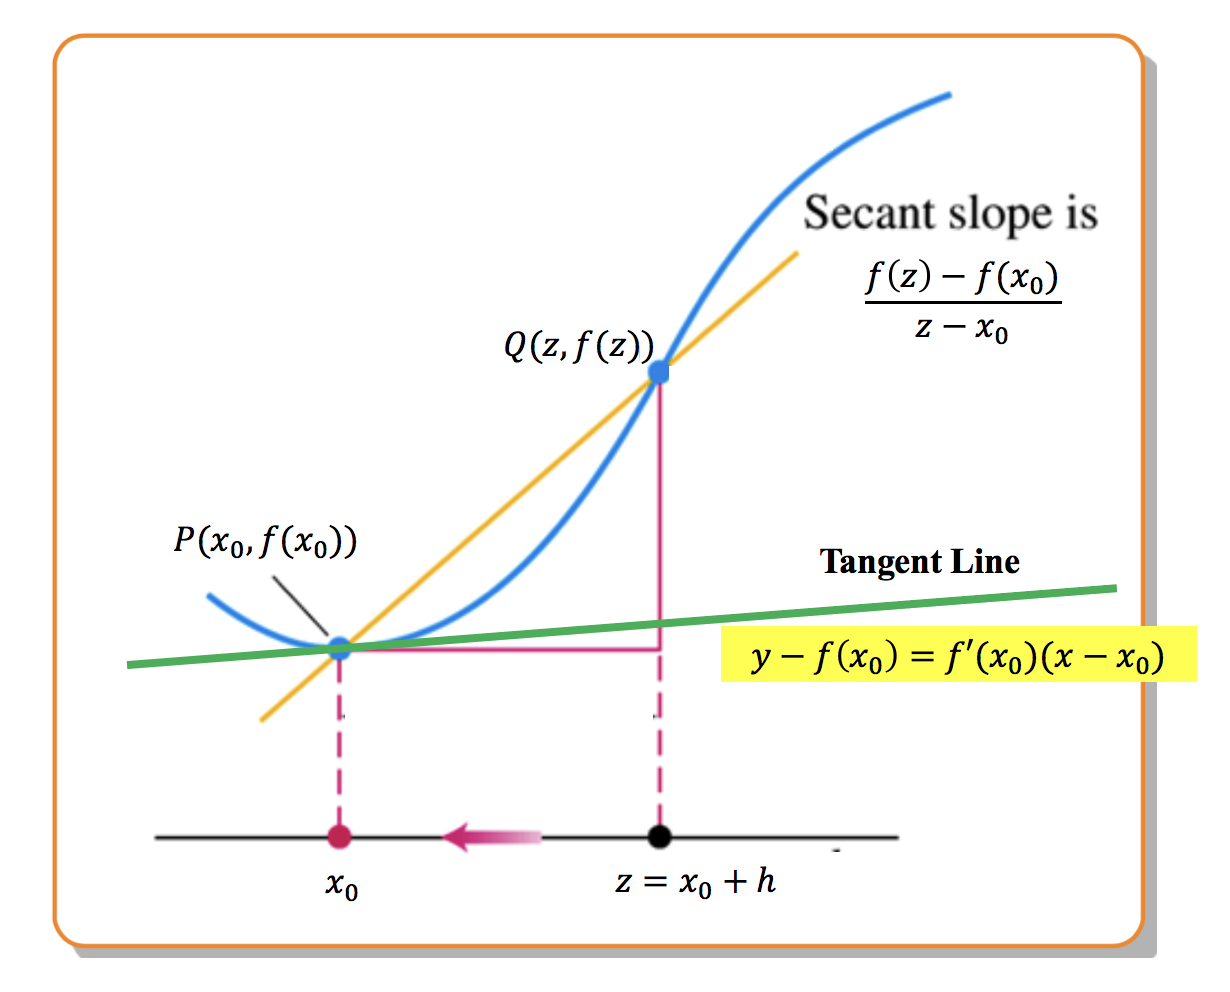
\includegraphics[width=10cm]{week5/de_2}
\caption{Interpretations of Derivative}
\end{figure}
Here the derivative is essentially the \emph{slope} of the tangent line to the curve $y=f(x)$ at $x=x_0$, where the tangent line is 
\[
y - f(x_0) = f'(x_0)(x-x_0)
\]
Here the tangent line is defined as the limit of secant line, i.e., taking limit $z\to x_0$, the secant line between $x_0$ and $z$ becomes the tangent line.


\paragraph{Arithmetic Insights of derivative}
The limit 
\[
f'(x_0):=\lim_{h\to0}\frac{f(x_0+h) - f(x_0)}{h},
\]
can be equivalently rewritten as:
\begin{itemize}
\item
$\left|\frac{f(x_0+h) - f(x_0)}{h}-f'(x_0)\right|\to0 (=o(1))$ as $h\to0$,
\item
$|f(x_0+h) - f(x_0) - f'(x_0)h|=o(h)\qquad\mbox{as }h\to0,$
\item
$f(x_0+h) = f(x_0) +f'(x_0)h+o(h)$ as $h\to0$. (useful equivalent definition for derivative)
\end{itemize}

Substituting $h=x-x_0$ into the above equation, we derive
\[
\begin{array}{ll}
|f(x) - [f(x_0) + f'(x_0)(x-x_0)]|=o(x-x_0),
&
\mbox{\textbf{Important Formula}}
\end{array}
\]
which essentially means that \textit{the differential provides the best linear approximation to the function in a neightborhood of a point}.
\subsection{Basic Rules of Differentiation}
Given two functions $g,f$, we study the derivative evaluated for the composite function $g\circ f$:
\begin{proposition}
$(g\circ f)'=g'(f(x))\cdot f'(x)$
\end{proposition}

Let's see how the engineer gives a proof: (recall MAT1001 slides, they exactly done this)
\begin{proof}[Engineers' proof]
Recall the definition
\[
(g\circ f)'(x):=\lim_{h\to0}\frac{(g\circ f)(x_0+h) - (g\circ f)(x)}{h}.
\]
Note that 
\[
\frac{(g\circ f)(x_0+h) - (g\circ f)(x)}{h}
=
\frac{(g\circ f)(x_0+h) - (g\circ f)(x)}{f(x+h) - f(x)}\frac{f(x+h) - f(x)}{h}.
\]
Taking the limit $h\to0$, the first term approaches $g'(f(x))$, and the second approaches $f'(x)$.
\end{proof}
\paragraph{Comments}
Note that $f(x+h) - f(x)$ may not be necessarily non-zero, and there is meaningless to pick a zero term in denominator.
\begin{proof}[Mathematicians' Proof]
Recall the definition
\[
(g\circ f)(x+h) - (g\circ f)(x)
:=
g(f(x)+f'(x)h+o(h)) - g(f(x))
\]
The differentiablity of $g$ gives us $g(y) = g(y_0) + g'(y_0)(y-y_0)+o(y-y_0)$, and therefore
\begin{align*}
(g\circ f)(x+h) - (g\circ f)(x)
&=
g(f(x)+f'(x)h+o(h)) - g(f(x))\\
&=\left\{g(f(x)) + g'(f(x))\left[(f'(x)h)+o(h)\right]\right\}-g(f(x))\\
&=g'(f(x))f'(x)h+\underbrace{g'(f(x))}_{\text{fixed as $x$ is fixed}}o(h)=g'(f(x))f'(x)h+o(h),
\end{align*}
\end{proof}
and therefore $(g\circ f)'(x)=g'(f(x))f'(x)$.

\subsection{Analysis on Differential Calculus}
\paragraph{Differentiablity implies continuity}
\begin{proposition}
If $f$ is differentiable at $x_0$, then it is continuous at $x_0$.
\end{proposition}
\begin{proof}
By definition of differentiablity,
\[
f(x)-f(x_0)=f'(x_0)(x-x_0)+o(x-x_0).
\]
Taking the limit $x\to x_0$, the RHS approaches 0, i.e., $\lim_{x\to x_0}f(x)=f(x_0)$.
\end{proof}


\begin{theorem}[Rolle's Theorem]
Suppose $f$ is differentiable on $[a,b]$, then $f'(x_0)=0$ if $x_0\in (a,b)$ is a local maximum or local minimum.
\end{theorem}
\begin{proof}
Note that
\[
f'(x_0)=\lim_{x\to x_0}\frac{f(x) - f(x_0)}{x-x_0}
\]
Suppose that $x_0$ is a local maximum, then
\begin{itemize}
\item
$x>x_0$ and $x$ close to $x_0$ implies $f(x) -f(x_0)\le0$, i.e., $\lim_{x\to x_0+}\frac{f(x) - f(x_0)}{x-x_0}\le0$
\item
Similarly, $x<x_0$ and $x$ close to $x_0$ implies $\lim_{x\to x-}\frac{f(x) - f(x_0)}{x-x_0}\ge0$.
\end{itemize}
Therefore 
\[
f'(x_0)=\lim_{x\to x_0}\frac{f(x) - f(x_0)}{x-x_0}=
\lim_{x\to x_0+}\frac{f(x) - f(x_0)}{x-x_0}
=
\lim_{x\to x-}\frac{f(x) - f(x_0)}{x-x_0}=0.
\]
\end{proof}
\begin{remark}
Geometrically this theorem is obvious. It asserts that at an extreme point of a differentiable function, the tangent line to its graph is horizontal.
\end{remark}

\paragraph{Estimation on finite increments}
The following two proposition are the most frequently used and important methods of studying numerical-valued functions.
\begin{theorem}[Mean-Value Theorem]
Suppose $f$ is differentiable on $[a,b]$, then there exists a point $c\in (a,b)$ such that
\[
\frac{f(b) - f(a)}{b-a}=f'(c)
\]
\label{The:5:2}
\end{theorem}
The proof relies on Rolle's theorem, i.e., we need to construct a function $h$ on $[a,b]$ that has a interior local maximum or local minimum. This is one useful trick.
\begin{proof}
We set $g(x) = \frac{f(b)  - f(a)}{b-a}(x-a)+f(a)$, i.e., $g$ is a secant line between $(a,f(a))$ and $(b,f(b))$. Then we consider the auxiliary function $h(x)=f(x)-g(x)$, which implies $h(a)=h(b)=0$.
\begin{itemize}
\item
If $h\equiv0$, then $g\equiv f$, and therefore $g'\equiv f'$, i.e., 
\[
g'(x)=\frac{f(b) - f(a)}{b-a}=f'(x), \qquad\forall x\in(a,b)
\]
\item
Otherwise, $h$ is positive or negative somewhere in $(a,b)$. w.l.o.g., $h$ is positive somewhere in $(a,b)$. Thus $h$ assumes its maximum in $(a,b)$, say $c$ (Exercise $\#$ 1). By rolle's theorem $h'(c)=0$, which impleis $f'(c) = g'(c)=(f(b) - f(a))/(b-a).$
\end{itemize}
\end{proof}
Applying Mean-Value Theorem, we give a more useful verison of Rolle's Theorem:
\begin{corollary}[Rolle's Theorem verison $2$]
Suppose $f$ is differentiable on $[a,b]$ with $f(a)=f(b)$, then there exists a point $c\in(a,b)$ such that $f'(c)=0$.
\label{Cor:5:1}
\end{corollary}
\begin{proof}
By Mean-Value Theorem,
\[
f(b)-f(a)=0=f'(c)(b-a)\implies f'(c)=0.
\]
\end{proof}

\paragraph{Exercise Verification}
Recall the proposition we have learnt:
\begin{proposition}
The range of a continuous function over a compact set is also compact.
\end{proposition}

As a result, $\sup_{x\in[a,b]}h=\max_{x\in[a,b]}h$, i.e., $h$ assumes its maximum in $[a,b]$.
\begin{remark}
Mean Value Theorem is correct, but not precise, i.e., 
we obtain an estimate of a function using affine. Now we are interested in approximations of a function by a polynomial $P_n(b)=P_n(b;a)=c_0+c_1(b-a)+\cdots+c_n(b-a)^n$. The Taylor's theorem gives the answer using integrals.
\end{remark}

\begin{theorem}[Taylor's Theorem]
Let $f$ be $n$ times differentiable on the open interval with $f^{(n-1)}$ continuous on the closed interval between $a$ and $x$, then
\[
f(x) = f(a)+f'(a)(x-a)+f''(a)\frac{(x-a)^2}{2!}+\cdots+f^{(n-1)}(a)\frac{(x-a)^{n-1}}{(n-1)!}+R_n(x),
\]
where the remainder is given by:
\[
R_n(x)=\frac{1}{(n-1)!}\int_a^xf^{(n)}(t)(x-t)^{n-1}\diff t
\]
\end{theorem}
\begin{proof}
All techniques in this proof is \emph{integration by parts}:
\begin{align*}
f(x) &= f(a)+\int_a^xf'(t)\diff t=f(a)-\int_a^xf'(t)\diff (x-t)\\
&=f(a)-f'(t)(x-t)|_{b}^{a}+\int_a^xf''(t)\diff t=f(a)+
f'(a)(x-a)+\int_a^x(x-t)f''(t)\diff t
\end{align*}
Applying the similar trick gives the result.
\end{proof}
\paragraph{Motivation of Continuosly differentiable}
\begin{remark}
If $f'(x_0)>0$, then $f$ is increasing at $x_0$. However, it does not mean that $f$ is increasing in a neighborhoold of $x_0$. That's because $f'$ may not be continuous.
\end{remark}
Some mathematicians give an example of a function that is everywhere differentiable but nowhere monotone:
\begin{example}
There exists a function haing the following properties:
\begin{enumerate}
\item
$f$ is differentiable with $|f'|\le1$ on $\mathbb{R}$
\item
Both $\{x\in\mathbb{R}\mid f'(x)>0\}$ and $\{x\in\mathbb{R}\mid f'(x)<0\}$ are dense in $\mathbb{R}$
\item
$\{x\in\mathbb{R}\mid f'(x)=0\}$ is also dense in $\mathbb{R}$
\item
$f$ is the difference of 2 monotone functions
\item
$f'$ is \emph{not} Riemann integrable.
\end{enumerate}
\begin{verbatim}
Reference: http://citeseerx.ist.psu.edu/viewdoc/download?
doi=10.1.1.843.5011&rep=rep1&type=pdf
\end{verbatim}
\end{example}
In the future when handling such topic, we will assume $f$ is \emph{continuously differentiable}, denoted as $f\in\mathcal{C}^1$. Then the example above will not appear.









